\section{Wall}
Wall-widgetten skal have mulighed for at oprette/slette/redigere en opslagstavle(Wall) og oprette/slette/redigere opslag (WallPost) til en specifik opslagstavle. Disse er essentielt set alle CRUD operationer. Desuden skal en opslagstavle kunne deles mellem flere grupper.

\subsection{Data view}
Indledningsvist oprettes to entitieter - Wall og WallPost, som bruges til at lave en tabel i databasen. Der er blevet besluttet at lave følgende struktur i databasen som kan ses på figur \ref{fig:Wall_ERDiagram}. På denne måde vil det blive muligt at tilføje WallPosts til en Wall, samt at oprette en Wall-widget.

\begin{figure}[H]
  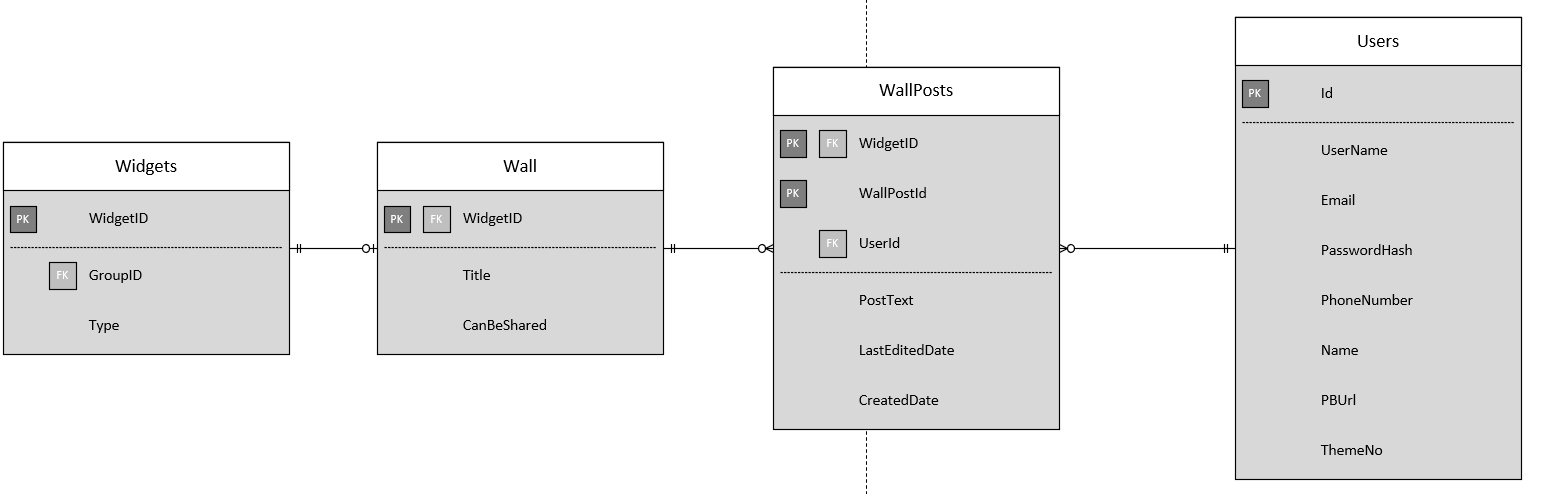
\includegraphics[width=1.0\linewidth]{01_Billeder/09_Arkitektur/Wall_DBArch.png}
  \caption{Færdige ER diagram over Wall. Denne strukture udvikles i 2. iteration, og forbliver den samme igennem udviklings processen. }
  \label{fig:Wall_ERDiagram}
\end{figure}

\jonathan{Du kunne godt trække Users lidt tættere på WallPosts så billedet kan blive lidt større?}

US'en der omhandler at kunne dele en opslagstavle med en anden grupper er der ikke lavet arkitetur for, da arbejdet på denne US ikke er påbegyndt endnu. Her ville det kræve at der blev oprettet en GroupsWalls tabel, der indeholder informationer om hvilke grupper der kan se hvilke Walls. 

\subsection{Logical view}
Logikken for denne del af systemet er forholdsvist simpel, og beskrives uddybende i bilag. Her er der dog lagt vægt på at brugere kun skal kunne tilgå de dele af Wall som de har tilgang til. Fx, skal det ikke være muligt for en hvilken som helst bruger at slette en anden brugers WallPost. I iteration 6, opdateres alt funktionalitet der opretter/sletter eller redigerer i enten WallPost eller Wall, til at vises i pop-up vinduer. Funktionaliteten i denne widget er forholdsvist lille, hvormed vurderes det at alt funktionaliteten kan tilgås fra widgetten på dashboard siden, uden at det bliver for uoverskueligt. Den færdige STM der bekriver de forskellige views og hvordan der kan laves om i dette, kan ses på figur \ref{fig:Wall_STM}.    

\begin{figure}[H]
  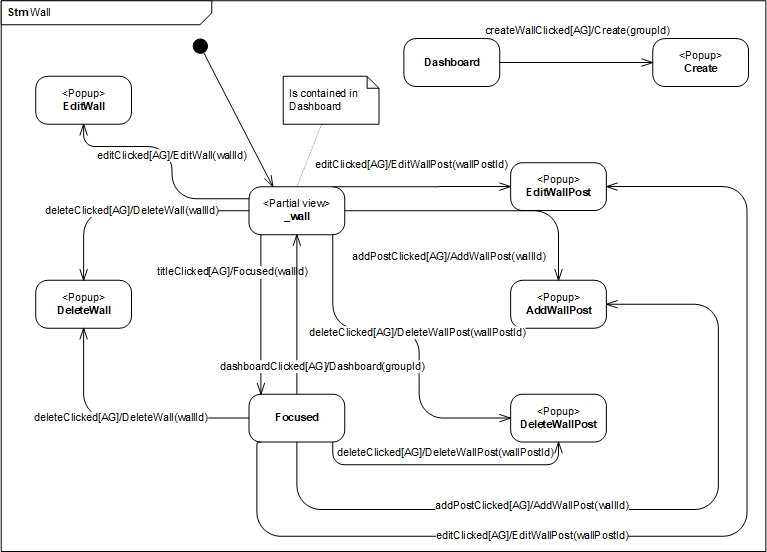
\includegraphics[width=1.0\linewidth]{01_Billeder/09_Arkitektur/Wall_STM.jpg}
  \caption{STM fra 6. iteration der viser hvordan der kan navigeres mellem forskellige views for at slette/redigere/oprette Wall, samt WallPosts. Når der trykkes på 'submit' knappen i et pop-up, laves der et postkald til en funktion af samme navn i WallControlleren. Herefter omdirigeres til det view som pilen peger på. Ordforklaring: AG - Access Granted}
  \label{fig:Wall_STM}
\end{figure}













